\chapter{Analiza danych}
\label{ch:analiza}

W niniejszym rozdziale przedstawiono wyniki modelowania cen energii za pomocą czterech modeli: regresji liniowej, regresji Ridge, Propheta oraz MLP. Analiza została podzielona na dwa podrozdziały, odpowiadające okresom stabilnemu i niestabilnemu. Zbiór danych został poddany testom w celu oceny skuteczności. W związku z tym dla każdego modelu przeprowadzono strojenie hiperparametrów. 

\section{Okres stabilny}
\label{sec:okres_stabilny}

\subsubsection{Regresja liniowa i Ridge}

Przeanalizowano modele regresji liniowej oraz regresji Ridge na danych z okresu stabilnego. Modele trenowano na danych z lat 2016--2018, a testowano na danych z 2019 roku.

Wyniki dla pełnego zbioru o 56 parametrach wejściowych przedstawiono w tabeli~\ref{tab:linear_ridge_results_full}. Regresja Ridge osiągnęła lepsze wyniki niż regresja liniowa, co jest widoczne w tabeli poniżej na podstawie przedstawionych wcześniej metryk ~ref/{sec:ocena_jakosci_prognoz}. Wynika to z powodu regularyzacji L2 zastosowanej w modelu Ridge. 

\begin{table}[h]
    \centering
    \caption{Wyniki regresji liniowej i Ridge dla pełnego zbioru danych w okresie stabilnym (2019).}
    \label{tab:linear_ridge_results_full}
    \begin{tabular}{|l|ccccc|}
        \hline
        \textbf{Model} & \textbf{MAE} & \textbf{RMSE} & \textbf{MAPE (\%)} & \textbf{sMAPE (\%)} & \textbf{\(R^2\)} \\
        \hline
        Regresja liniowa & 16.41 & 21.19 & 8.17 & 7.60 & 0.8178 \\
        Regresja Ridge   & 16.07 & 20.62 & 7.96 & 7.46 & 0.8275 \\
        \hline
    \end{tabular}
\end{table}

Najlepsza wartość hiperparametru \(\alpha\) w regresji Ridge wyniosła 500.0. Wysoka wartość \(\alpha = 500.0\) sugeruje, że w pełnym zbiorze danych występuje istotna współliniowość między zmiennymi objaśniającymi. Może to być spowodowane wysoką korelacją między zmiennymi, np. zmiennymi pogodowymi.

Następnie przeprowadzono analizę skróconego zbioru danych opisanego w ~\ref{sec:shortened_dataset}. Wyniki dla skróconego zbioru danych przedstawiono w tabeli ~\ref{tab:linear_ridge_results_short}, wraz z różnicami w metrykach względem pełnego zbioru danych. Wyniki dla skróconego zbioru były nieco gorsze: dla regresji Ridge MAPE wyniosło 8.15\% w porównaniu do 7.96\% dla pełnego zbioru, a \(R^2\) spadło z 0.8275 do 0.8144. Różnice w metrykach wskazują, że dodatkowe zmienne w pełnym zbiorze danych wnoszą istotną informację, mimo niższego poziomu korelacji ze zmienną objaśnianą. Jednak różnice nie są bardzo duże (np. MAPE różni się o 0.19\% dla regresji Ridge), co może sugerować, że skrócony zbiór danych nadal zawiera najważniejsze zmienne objaśniające.

\begin{table}[h]
    \centering
    \caption{Wyniki regresji liniowej i Ridge dla skróconego zbioru danych w okresie stabilnym (2019) wraz z różnicami względem pełnego zbioru.}
    \label{tab:linear_ridge_results_short}
    \begin{tabular}{|l|ccccc|c|}
        \hline
        \textbf{Model} & \textbf{MAE} & \textbf{RMSE} & \textbf{MAPE (\%)} & \textbf{sMAPE (\%)} & \textbf{\(R^2\)} & \textbf{Różnica MAPE (\%)} \\
        \hline
        Regresja liniowa & 17.57 & 22.20 & 8.54 & 8.02 & 0.8001 & +0.37 \\
        Regresja Ridge   & 16.73 & 21.39 & 8.15 & 7.69 & 0.8144 & +0.19 \\
        \hline
    \end{tabular}
\end{table}

W celu potencjalnego polepszenia wyników zastosowano logarytmizację zmiennej wyjściowej (\texttt{fixing\_i\_price}), co miało na celu zmniejszenie skośności rozkładu cen i poprawę dopasowania modelu. Wyniki z logarytmizacją przedstawiono w tabeli~\ref{tab:linear_ridge_results_log}.

\begin{table}[h]
    \centering
    \caption{Wyniki regresji liniowej i Ridge z logarytmizacją dla okresu stabilnego (2019).}
    \label{tab:linear_ridge_results_log}
    \begin{tabular}{|l|ccccc|}
        \hline
        \textbf{Model i zbiór danych} & \textbf{MAE} & \textbf{RMSE} & \textbf{MAPE (\%)} & \textbf{sMAPE (\%)} & \textbf{\(R^2\)} \\
        \hline
        Regresja liniowa (pełny)   & 21.63 & 28.36 & 9.85 & 9.16 & 0.6736 \\
        Regresja Ridge (pełny)     & 19.99 & 26.06 & 9.21 & 8.65 & 0.7244 \\
        Regresja liniowa (skrócony) & 26.36 & 33.07 & 11.95 & 10.94 & 0.5563 \\
        Regresja Ridge (skrócony)   & 23.29 & 29.38 & 10.69 & 9.89 & 0.6498 \\
        \hline
    \end{tabular}
\end{table}

Logarytmizacja nie przyniosła spodziewanych korzyści i pogorszyła wyniki we wszystkich metrykach. Największe pogorszenie zaobserwowano dla skróconego zbioru danych, gdzie MAPE dla regresji liniowej wzrosło do 11.95\%, a \(R^2\) spadło do 0.5563. Przyczyną jest najprawdopodobniej fakt, że rozkład cen w okresie stabilnym nie jest mocno skośny ze średnią wynoszącą 193,51 PLN oraz medianą 182 PLN, więc logarytmizacja wprowadziła niepotrzebne nieliniowości, które utrudniły dopasowanie modeli liniowych. Dodatkowo, odwrócenie transformacji logarytmicznej może amplifikować błędy predykcji, co wpłynęło na wzrost RMSE i MAE.

Wyraźne jest, że regresja Ridge w porównaniu do regresji liniowej lepiej radzi sobie z danymi o dużej liczbie zmiennych objaśniających, co potwierdzają wyniki dla pełnego zbioru danych. Poniżej przedstawiono wykresy rzeczywistych i przewidywanych wartości.

\begin{figure}[H]
    \centering
    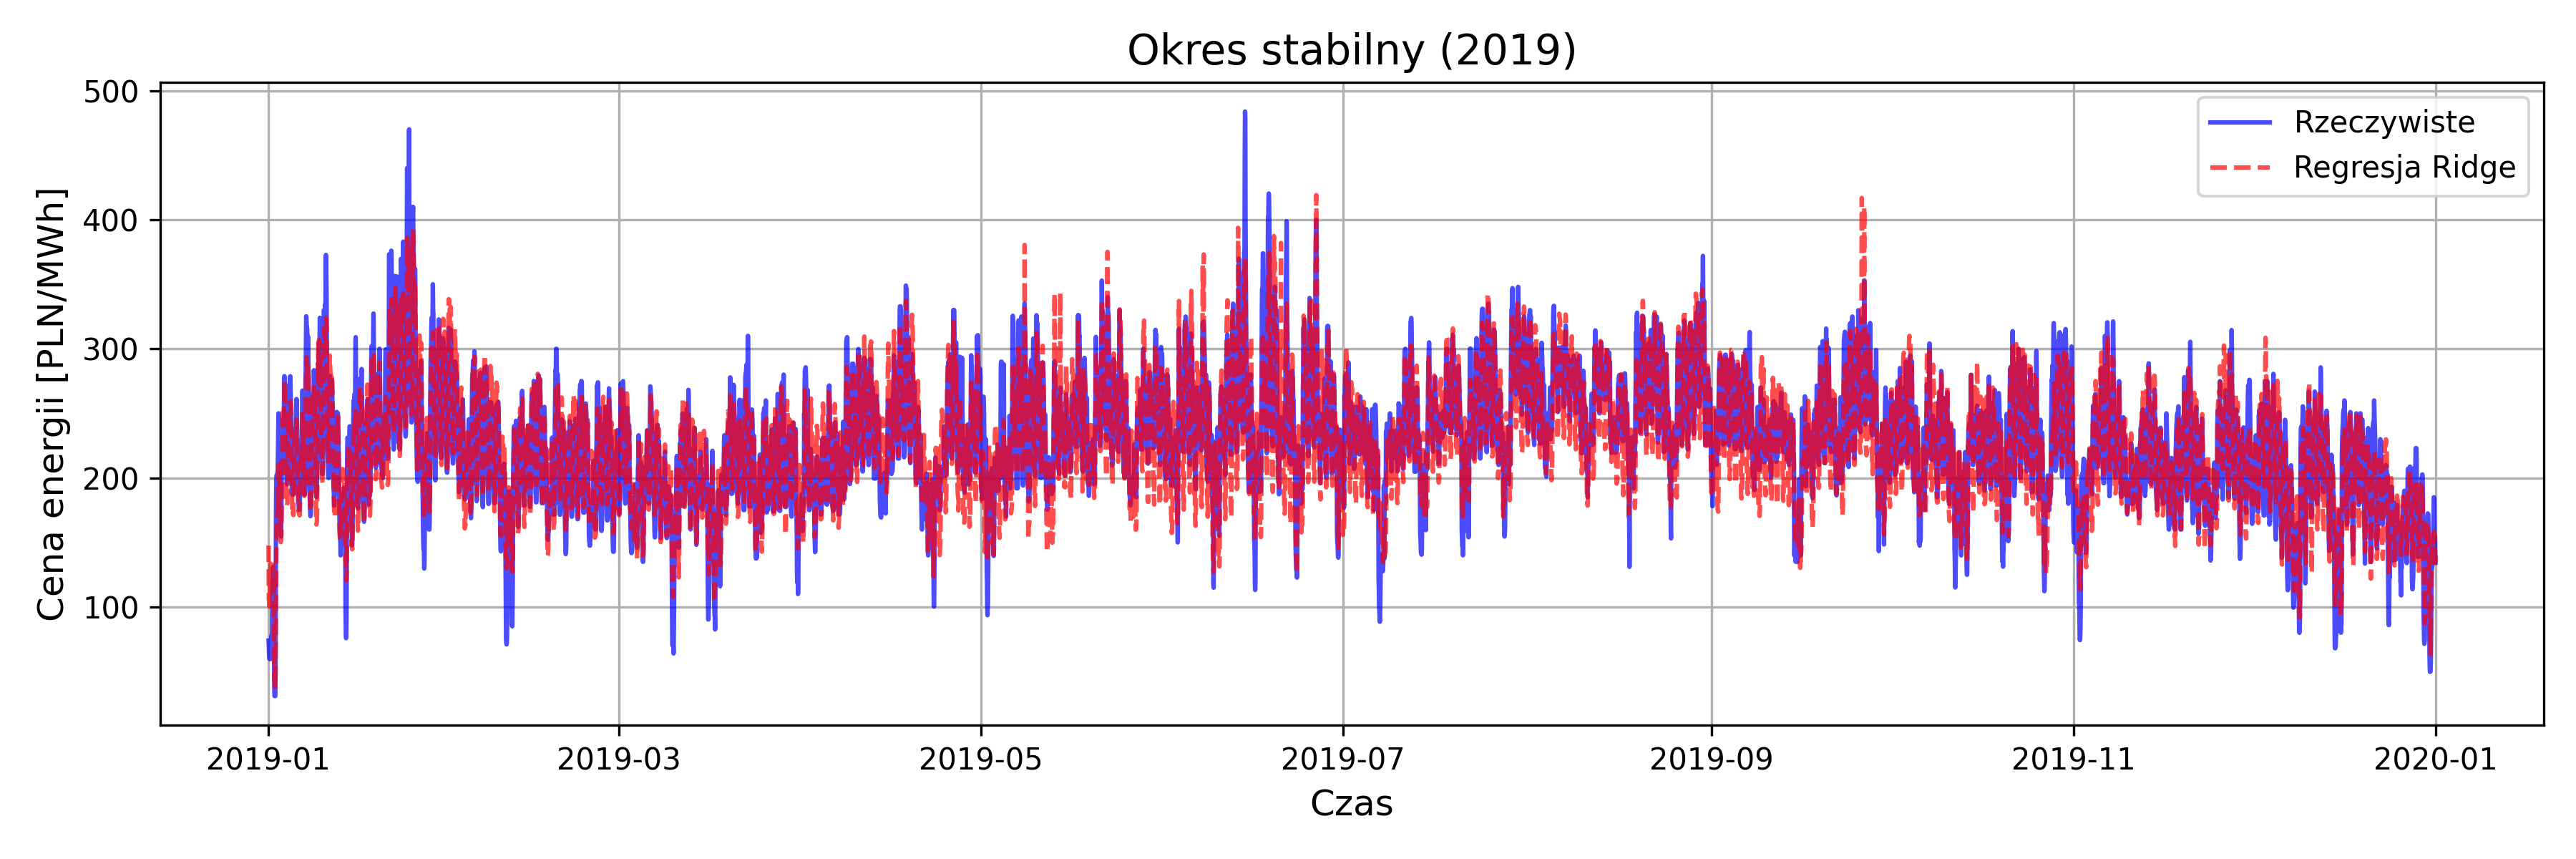
\includegraphics[width=1.0\textwidth]{../../plots/predicts/ridge_predictions_full_stable_period.png}
    \caption{Porównanie rzeczywistych i przewidywanych wartości cen energii dla regresji Ridge w okresie stabilnym.}
    \label{fig:ridge_predictions_full_stable_period}
\end{figure}

Widoczne na wykresie jest to, że model nie nadąża za zbyt wysokimi bądź zbyt niskimi wartościami. Może to sugerować, że model nie jest wystarczająco elastyczny, aby uchwycić te zmiany. Wartości przewidywane przez model są bardziej liniowe od rzeczywistych cen energii, co jest typowe dla modeli regresyjnych.

W związku z tym, przygotowany został histogram reszt dla regresji Ridge, aby ocenić, czy reszty są rozkładem normalnym. 

\begin{figure}[H]
    \centering
    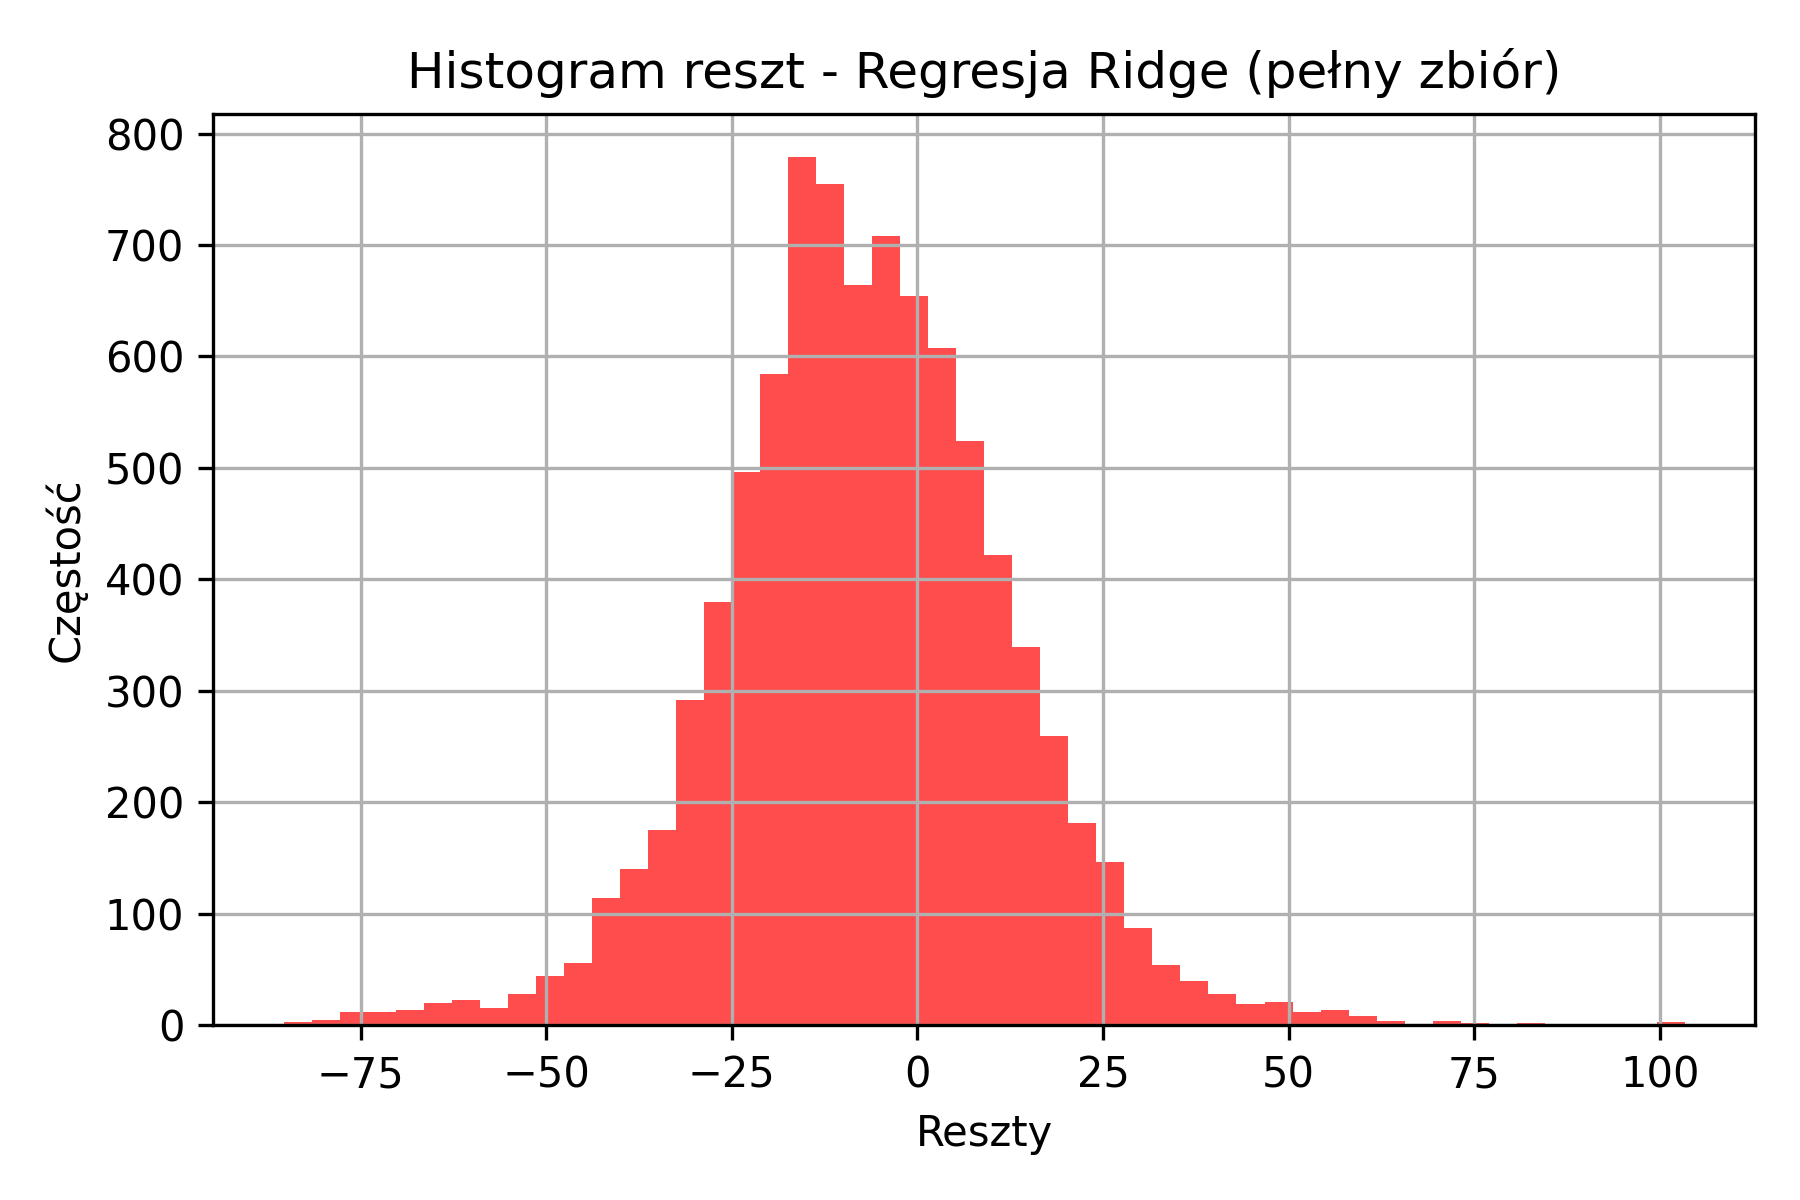
\includegraphics[width=1.0\textwidth]{../../plots/predicts/residuals_histogram_Ridge_full_stable_period.png}
    \caption{Histogram reszt dla regresji Ridge w okresie stabilnym.}
    \label{fig:ridge_residuals_full_stable_period}
\end{figure}

Histogram posiada jeden ze szczytów w okolicy zera i większość reszt skupia się w okolicy zera. Rozkład reszt jest zbliżony do normalnego, ale jest asymetryczny w lewą stronę, co może sugerować, że model jest skłonny do niedoszacowywania wartości. Potwierdza się teza z wykresu rzeczywistych i przewidywanych wartości, która sugeruje, że znajdują się obserwacje z dużymi resztami zarówno dodatnimi, jak i ujemnymi.

\section{Okres niestabilny}
\label{sec:okres_niestabilny}

Rigde : W pracy wartość \( \lambda \) została wybrana na podstawie walidacji krzyżowej (ang. cross-validation), aby zoptymalizować równowagę między dopasowaniem modelu do danych a jego zdolnością do generalizacji.